\chapter{Solution}
\label{ch:solution}

\section{Requirements}

The requirements in this project were to simulate a dynamic crisis environment and to discover whether ant colony optimization would perform better than Dijsktra's pathfinding algorithm in this environment. The dynamic crisis environment, the ship models, needs to adequately represent reality. However the models does not need to be detailed to the point where chairs and people are shown within the rooms. Passengers will spend a fixed amount of time crossing the different types of rooms thus defeating the purpose of creating a highly detailed model. 

The fire, one of the dynamic elements in the simulation, will be modeled fairly simplistic. It only needs to create changes in the model, thus forcing the pathfinding algorithms to find new paths, or decide it is best to stay on the current one. The fire starting will be the first step in the simulation. As the fire grows in size it will spread faster. It will have to spread faster between floors then along them. 

In the simulation all passengers needs to be tracked and accounted for. Additionally all passengers needs to be able to follow directions. The passengers needs to follow basic human behavior patterns. For instance they may panic in the face of danger or start searching for family members, both of which would mean that the passenger is ignoring directions.

\section{Implementation}

\subsection{Ship Model}

\begin{figure} [h]
\centering
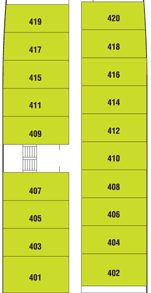
\includegraphics[angle=90]{images/rooms.png}
\caption{A small section of a ship deck}
\label{fig:rooms}
\end{figure}

\begin{figure} [h]
\centering
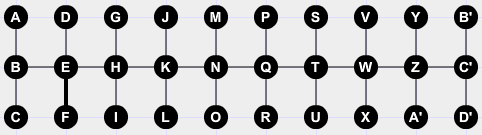
\includegraphics{images/simple.png}
\caption{The graph representing the ship deck}
\label{fig:simple}
\end{figure}

The ships are created from blueprints from ships currently in operation. They are modeled as graphs, nodes represents rooms and lines represents passages between rooms. Small rooms are represented by a single node as the layout of the room is fairly simplistic and the time it takes to move across the room is fairly predictable as long as the room is not crowded. Figure \ref{fig:rooms} shows a section of a ship deck with several rooms leading out into a hallway connected to a set of stairs. Figure \ref{fig:simple} shows a graph representing the same section. It is worth noting that while small rooms can be represented with a single node the hallway is represented by multiple nodes as a passenger exiting room 419 is far away from a passenger exiting room 401.

Complex or large rooms are represented by multiple interconnected nodes so each part of the room can be individually configured to better represent the room. Rooms like the dining room in the MS Reflection, as seen in figure \ref{fig:dining}, would need several nodes as the time it takes for the people close to the exit to evacuate are vastly different from the time it takes for the people sitting in the middle of the room to evacuate. Figure \ref{fig:complex} shows a representation of the dining room. 

\begin{figure} [h]
\centering
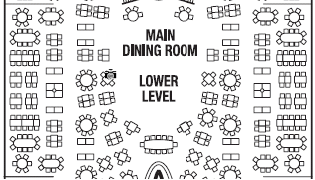
\includegraphics{images/Dining.png}
\caption{The dining room in the cruise ship MS Reflection}
\label{fig:dining}
\end{figure}

All rooms have a few characteristics associated with them. First is the room capacity, meaning the amount of people that can move across the room before they start to slow each other down. Second is the chance of death, this number will change over time as the fire spreads throughout the ship. Third is the type of room, for instance stairs, hallway, gift shop etc. Fourth is the size of the room, which in turn will determine the time it takes to traverse the room. Additionally there are a exit nodes where all passengers gather before lifeboat embarkation. These are the nodes the algorithms attempts to guide the passengers towards.

\begin{figure} [h]
\centering
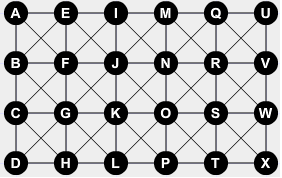
\includegraphics{images/complex.png}
\caption{A simple representation of the dining room of the MS Reflection}
\label{fig:complex}
\end{figure}

It became clear to us that using pathfinding algorithms to find the shortest route of small vessels were unnecessary as  there often would be only a single route to take and all passengers would be confined to one or two large areas where personnel easily could guide the passengers to safety. The algorithms are only helpful given multiple routes and rooms. 

\subsection{Human Behavior}

% Varying chance of panic

At the beginning of the simulation we assume that all passengers have access to a smart phone, which will show them the way out, and that they are following directions. Additionally, no passengers will start the simulation in a panicked state. However at certain time intervals a check is made to determine whether a passenger panics or not. Close proximity to fire, a high density of passengers or other panicked passengers increase the chance that they themselves will panic. When in a panicked state the passengers run out of the ship the same way they walked into it. Even if that path is significantly more dangerous.

Passengers with family members onboard the ship can enter a search state where they walk in a random pattern searching for family members until they find them, at which point they can resume following directions. The passengers can spot family members within their own node and any adjacent nodes. Family members that are not in a search state will also group up if they are within spotting range. In this case the family member that is further along the escape path will wait for the other family member to catch up.

Furthermore, family members will stick together and the algorithms will make no attempts to split up a family and send them in multiple directions. Thus whenever a passenger is moved the program checks if a family member is close-by, and if so they are moved in the same direction.

\subsection{Algorithms}
The simulation starts by igniting between one and three fires. There is a time delay between the time the fire starts and the time the passengers begins to move. This delay is meant to account for the time it takes to react to the alarm, retrieve the smart phone and understand the directions given. Fires spreads faster between floors than along them. The speed of the fire depends on the ship materials and access to oxygen, thus we run the simulations with varying speeds to observe how the algorithms perform. The larger the fire is, the faster it spreads to the neighboring nodes. Additionally deadly smoke will spread further and faster than the fires. 

When the fire starts either the fire system is able to track the position of the fire or the electric system have been compromised and the ship is in a dead ship condition where tracking the progress of the fire is impossible. If there are no information about the location of the fire then the safest possible route is likely the quickest one. Thus we decided upon 4 different possible configurations of the algorithms, to test if different configurations perform better in different scenarios. First they can prioritize distance and selecting the shortest path. Second they can prioritize safety and completely ignore the distance to the exit. Third it can combine the two variables, valuing them equally or differently. Fourth it can first sort the paths based on one variable and then only sort based on the other variable if there is a tie. For instance if there are two equally safe paths the shortest one is chosen.

The speed of the passengers is based on two factors, the type of room and the amount of people in the room. Passengers in a crowded flight of stairs will move significantly slower than a passenger in an empty corridor. These numbers are gathered from IMO's estimation on passenger speed during evacuations \cite{speed}. Given a node of 4 meter length and a passenger speed of 1 m/s the passenger will naturally have traversed the node after 4 seconds. It is worth mentioning that the passenger will not move within the node itself, up to 4 seconds into the simulation the passenger is located in the initial node and at 4 seconds the passenger is then moved to the next node.










